\documentclass[a4paper]{oblivoir}
% define the title
\author{Moon Il-chul \\ \href{mailto:icmoon@kaist.ac.kr}{icmoon@kaist.ac.kr} 
   \and Hwang Gyeong-jo \\ \href{mailto:hkj4276@kaist.ac.kr}{hkj4276@kaist.ac.kr} }
\setcounter{chapter}{2}
\title{Chapter 2. Fundamentals of Machine Learning}
\usepackage{indentfirst}
\usepackage{graphicx}
\graphicspath{ {Figure/} }
\usepackage{hyperref}
\usepackage{amsmath}
\usepackage{amssymb}
\usepackage{amsfonts}
\usepackage{dsfont}
\usepackage[]{algorithm2e}
\usepackage{chngcntr}
\counterwithin{figure}{chapter}
\setcounter{tocdepth}{2}
\setcounter{secnumdepth}{3}
\hypersetup{pdfborder={0 0 0}}
\renewcommand{\thefigure}{\thechapter-\arabic{figure}}
\renewcommand{\theequation}{\thechapter.\arabic{equation}}
\newlength\myindent
\setlength\myindent{5em}

\begin{document}
% generates the title
\maketitle
%\renewcommand{\contentsname}{목차}
\tableofcontents
%\listoftables
%\listoffigures

%슬라이드 3
\section{규칙기반(Rule-based) 학습}

%슬라이드 4
\subsection{복습}
Tom M. Mitchell 교수는 다음과 같이 기계학습을 정의하였다; \textit{컴퓨터 프로그램이 특정 업무(Task) $T$를 수행함에 있어서, 평가지표(Performance Measure)인 $P$의 값이 경험(Experience) $E$를 통해 개선될 때, 이 \textbf{프로그램이 학습한다}고 말한다.}\\
(A computer program is said to learn from experience $E$ with respect to some class of tasks $T$ and performance measure $P$ if its performance at tasks in $T$, as measured by $P$, improves with experience $E$)\\
\indent 압정 던지기 실험에서 보았듯이, 더 많은 데이터가 있으면 그만큼 사전 지식(Prior Knowledge)이 쌓이게 되고, 이는 사후확률(Posterior Probability)을 더 정확히 추론하는데에 큰 도움을 준다. $a_{H}$, $a_{T}$를 각각 앞면이 나온 횟수, 뒤집힌 횟수라고 했을 때, Likelihood function은 Binomial Distribution을 따르고 $P(\theta)$는 Beta Distribution을 따른다고 가정하였다.\\
\indent 이 단원에서는 압정 던지기 실험에서 더 나아가 규칙기반적 접근(Rule-based Approach)에 대해 배워보고,  고전 통계학적 접근(Classical Statistics Approach), 정보이론적 접근(Information Theory Approach)에 대해 배워볼 것이다.\\

%슬라이드 5
\subsection{규칙기반 학습(Rule-based Learning)을 위한 이상세계}
다음의 가정을 만족시키는 이상세계(Perfect World)를 가정해보자.
\begin{itemize}
\item No observation errors, no inconsistent observations; 관측 오차나 비일관적인 데이터는 존재하지 않는다. 즉, 훈련(Training) 과정에서 사용할 데이터에는 잡음(Noise)이 없으며, 상호 모순적이지 않다.
\item No stochastic elements in the system we observe; 관측 대상이 되는 계에서 확률적인 요소는 존재하지 않는다. 다시 말해서, 결과에 영향을 미치는 요소들 중에서 주사위 놀이와 같이 확률적으로 영향을 주는 요소는 없다는 것이다. 따라서 모든 결과는 인과적(Causal)이며 결정론적(Deterministic)이다.
\item Full information in the observations to regenerate the system; 대상이 되는 계를 파악하기 위한 모든 정보가 주어져 있다. 즉, 주어진 데이터로 학습하여 알아낸 목표함수(Target Function)는 Hypothesis Set에 포함된다. \\
\end{itemize}

\indent 이상적인 세계에서 한 가족이 날씨의 상태와 일기예보 등에 따라 야외 물놀이를 즐겼는지 알아보자. 아래의 표에서 Sky, Temperature, Humidity, Wind, Water, Forecast는 각각 순서대로 하늘의 상태, 기온, 습도, 바람의 정도, 수온, 일기예보를 나타내고, Enjoy Sport는 밖에서 물놀이 스포츠를 즐겼는지 여부를 나타낸다. 아래의 테이블과 같은 관측 데이터를 Experience, 이를 통해 실제로 물놀이 스포츠를 즐기러 나갈지 여부를 예측하는 작업을 Task, 그리고 얼마나 잘 맞추는지를 Performance Measure라고 했을 때, 기계학습 알고리즘은 주어진 Experience로부터 학습하여 사람들이 나가서 물놀이를 즐길지 여부를 예측하는 것이다. \\
\indent 이 예제에서 위의 세 가지 가정은 다음과 같이 해석할 수 있다; 실생활에서는 날씨를 표현할 때 `맑음'인지 `구름 조금'인지 애매한 상황이 있을 수 있다면, 이 예제는 이상적인 세계이므로 이런 애매한 상태는 존재하지 않는다. 그리고 정확히 일치하는 두 가지 조건이 주어졌을 때, 하루는 밖에서 물놀이를 즐긴 반면, 하루는 나가서 놀지 않는 일관적이지 않은(inconsistent) 데이터는 존재하지 않는다. 또한 날씨 상황이 주어졌을 때, 나가서 놀던지 말던지 둘 중에 하나는 반드시 결정론적으로 정해지며, 이 과정에서 어떠한 Random effect도 관여하지 않는다. 마지막으로, 이 시스템을 설명하기 위해 필요한 모든 데이터는 주어져있다고 가정한다.
\begin{figure}[ht]
\centering
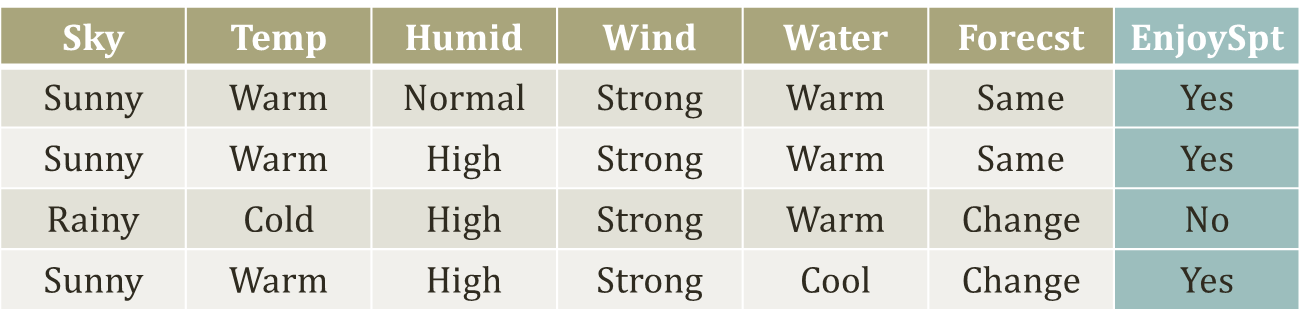
\includegraphics[scale=0.5]{Table1.png}
\caption{날씨나 기상예보에 따른 한 가족의 야외 물놀이 여부 데이터}
\label{Figure 2-1}
\end{figure}

%슬라이드 6
\subsection{Function Approximation}
위의 물놀이 예제에서 어떤 함수가 존재하여, 그 함수에 날씨의 상태를 변수로 입력하면 나가서 물놀이를 즐길지 말지를 결정할 수 있다면 어떨까? 이러한 의미에서 기계학습이란 주어진 데이터를 잘 설명하는 approximated function을 찾는 과정이라고 할 수 있다. \\
\indent 그렇다면 function approximation을 배우기 전에, 우선 다음과 같은 용어들을 정의하자.
\begin{description}
\item [Instance $X$] 인스턴스란, 하나의 Example 혹은 관측 집합을 말한다. 위의 표에서 하나의 행 전체가 인스턴스라고 볼 수 있다. 따라서 이 예제는 4개의 인스턴스로 이루어진 세계이다. 하나의 인스턴스는 다시 Feature와 Label로 나눌 수 있는데, 결과값인 Enjoy Sport를 Label, 그리고 Label을 결정하는 나머지 요소들을 Feature라고 한다. 
\item [Training Dataset $D$] 훈련 데이터란, 여러 개의 인스턴스를 모아놓은 집합을 말한다. 즉, 예제는 Sky, Temperature, Humidity, Wind, Water, Forecast 등 6개의 Feature와 하나의 Label인 Enjoy Sport로 이루어진 인스턴스 4개가 모여서 훈련 데이터를 구성한 것이다.
\item [Hypothesis $H$] 가설이란, 데이터를 그럴듯하게 설명할 수 있는 임의의 함수를 말한다. 이 예제에서는 $3^{6}$개의 가설이 존재한다.
\item [Target Function $c$] 목표 함수란, 우리가 실제로는 알지 못하지만, 주어진 데이터를 통해 추론하고자 하는 정답이라고 할 수 있다. 뒤에서 우리는 가장 세부적인 가설로부터 시작하여 이를 점차 일반화시키는 Generalization 방법과, 가장 일반적인 가설로부터 시작하여 이를 점차 구체화시키는 Specialization 방법에 대해 배워볼 것이다. \\
\end{description}

%슬라이드 7
\subsubsection{Function Approximation의 시각적 표현}
\begin{figure}[ht]
\centering
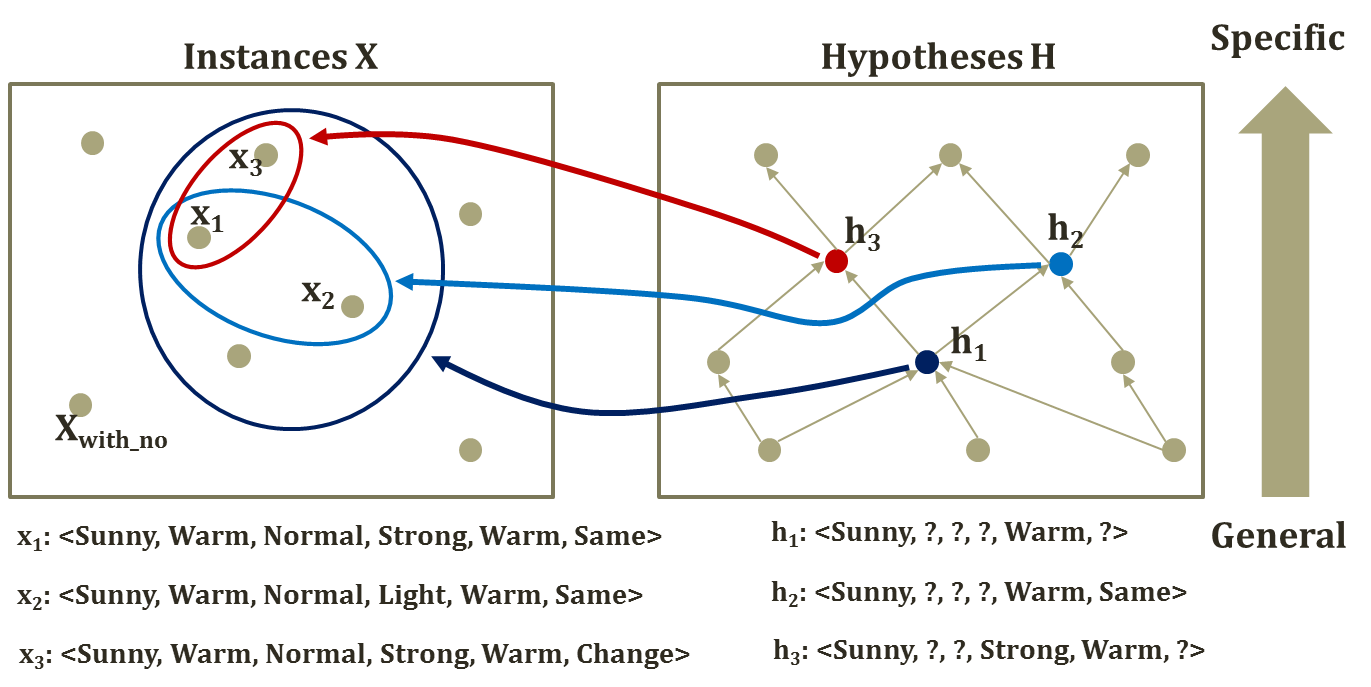
\includegraphics[scale=0.5]{Function_Approximation1.png}
\caption{Function Approximation의 시각적 표현}
\label{Figure 2-2}
\end{figure}

\indent 각각의 인스턴스 $x_{1}$, $x_{2}$, $x_{3}$는 이 그림에서 점으로 표현되었다. Hypothesis Space에서 $h_{1}$, $h_{2}$, $h_{3}$와 같은 점은 각각 어떠한 경우에 밖으로 물놀이를 나갈지에 관해 추측한 가설이다. ''?''는 해당 항목에 의해 영향을 받지 않는다는 뜻이다. 따라서 $h_{1}$은 ''하늘이 맑고 수온이 따뜻하면 무조건 나가서 놀 것이다.''는 가설이고, $h_{2}$는 $h_{1}$에서 더 나아가 ''하늘이 맑고 수온이 따뜻하며, 일기예보에서 날씨가 변하지 않을 것이라고 하면 나가서 놀 것이다.''는 가설이다. $h_{3}$는 ''하늘이 맑고 바람이 시원하게 불며, 수온이 따뜻하면 나가서 놀 것이다.''는 가설이다. \\
\indent 세 개의 인스턴스 $x_{1}$, $x_{2}$, $x_{3}$ 모두 맑은 하늘과 따뜻한 수온의 조건을 만족시키므로 가설 $h_{1}$은 모든 인스턴스를 포함한다는 것을 알 수 있다. 그리고 인스턴스 $x_{2}$는 가설  $h_{3}$의 바람 조건을 만족하지 못하고, 인스턴스  $x_{3}$는 가설 $h_{2}$의 일기예보 조건을 만족하지 못하는 것을 볼 수 있다. 따라서 위의 그림은 가설들과 인스턴스들 사이의 포함 관계를 함수로서 나타낸 그림이 되는 것이다. 여기서 $h_{1}$과 같이 필요한 조건들이 비교적 적은 가설을 일반적(General) 가설이라 표현하고, $h_{3}$와 같이 좀 더 많인 조건들이 필요한 가설을 구체적(Specific) 가설이라 표현한다. 따라서 General한 가설일수록 Instance Space에서 더 많은 원소들을 포함한다. \\

%슬라이드8
\subsection{Find-S Algorithm}
Find-S 알고리즘이란 가장 구체적인 가설로부터 시작하여 인스턴스들을 거치며 올바른 가설을 찾아가는 알고리즘이라 할 수 있다. 좀 더 설명하자면, \\
\indent\rule{10cm}{0.4pt} \\
\begin{algorithm}[H]
	\SetAlgoLined
	\KwData{Training Dataset}
	\KwResult{Find the Correct Hypothesis}
	Initialize $h = h_{0}$
	\For{instance $x$ in $D$}{
		\eIf{$x$ is positive}{
			\For{Feature $f$ in $O$}{
				\eIf{$f_{i}$ in $h == f_{i}$ in $x$}{
					Do Nothing;
				}{
					$f_{i}$ in $h = f_{i}$ in $h \cup f_{i}$ in $x$
				}
			}
		}{}
	}
\end{algorithm}

\indent \rule{10cm}{0.4pt} \\
\indent 우선 $h$를 가설 집합에서 가장 구체적인 가설로 두어 초기화시키고, 각각의 인스턴스 $x \in D$에 대해서 $x>0$이면 다음을 진행한다; 각각의 feature $f$에 대해서 $h$와 $x$의 $i$번째 feature가 일치한다면, $h$를 업데이트하지 않고 넘어간다. 반면 $h$와 $x$의 $i$번째 feature가 일치하지 않는다면, $h$의 feature를 $x$의 feature로 업데이트한다. 다음의 예시를 살펴보자
\begin{itemize}\setlength\itemsep{-\parsep}
	\item Instances
	\begin{description}\setlength\itemsep{-\parsep}
		\item [$x_{1}$]: $<$Sunny, Warm, Normal, Strong, Warm, Same$>$
		\item [$x_{2}$]: $<$Sunny, Warm, Normal, Light, Warm, Same$>$
		\item [$x_{4}$]: $<$Sunny, Warm, Normal, Strong, Warm, Change$>$
	\end{description}
\end{itemize}
\begin{itemize}\setlength\itemsep{-\parsep}
	\item Hypotheses
	\begin{description}\setlength\itemsep{-\parsep}
		\item [$h_{0}$]: $<\emptyset, \emptyset, \emptyset, \emptyset, \emptyset, \emptyset>$
		\item [$h_{1}$]: $<$Sunny, Warm, Normal, Strong, Warm, Same$>$
		\item [$h_{1,2,3}$]: $<$Sunny, Warm, Normal, ?, Warm, Same$>$
		\item [$h_{1,2,3,4}$]: $<$Sunny, Warm, Normal, ?, Warm, ?$>$
	\end{description}
\end{itemize}
\begin{figure}[ht]
\centering
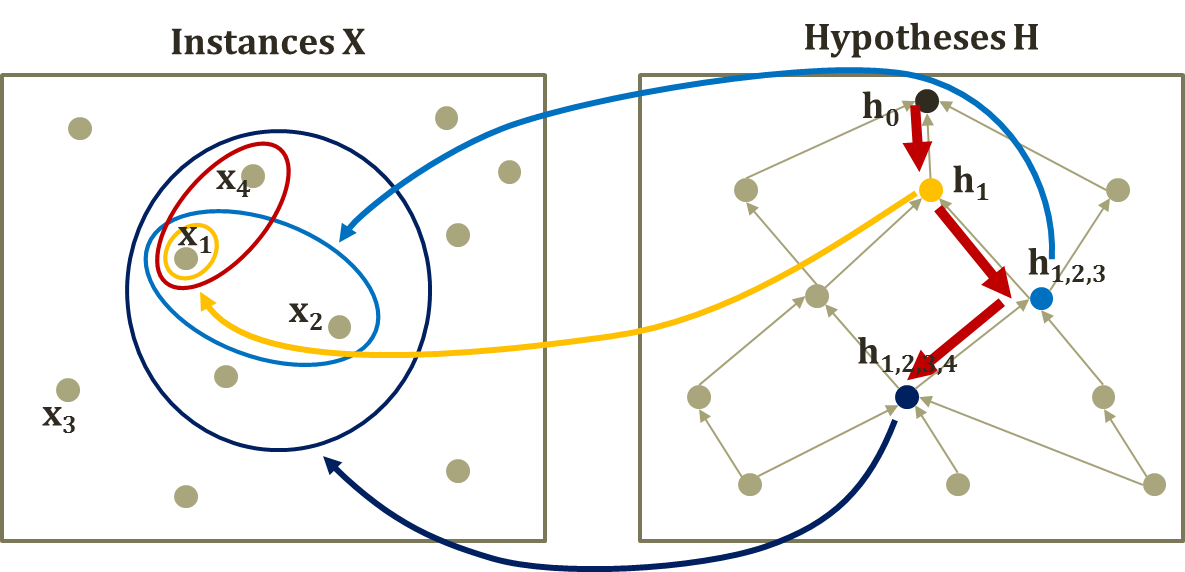
\includegraphics[scale=0.5]{Function_Approximation2.png}
\caption{Find-S 알고리즘 예시}
\label{Figure 2-3}
\end{figure}

%슬라이드9
\subsection{Version Space}
Find-S 알고리즘을 통해 목표함수를 찾아내기에는 너무나 많은 가설들이 존재하고, 이를 효과적으로 줄일 수 없다. 따라서, 가능한 가설들의 경계를 설정하는 것이 필요하다. 이를 Version Space라고 부르며, 주어진 데이터로부터 추론 가능한 모든 가설들의 집합으로 정의한다. \\
\indent \textbf{$VS$}(Version Space)의 원소들 중에서 가장 일반화된 가설들의 집합을 General Boundary라고 부르고, 이를 \textbf{$G$}라 표기한다. 이와 비슷하게, \textbf{$VS$}의 원소들중에서 가장 구체화된 가설들의 집합을 Specific Boundary라고 부르고, 이를 \textbf{$S$}로 표기한다. 이때, 임의의 가설 \textbf{$h$}$\in H$에 대하여 다음이 성립한다.
\begin{equation}
VS_{H, D} = \{ h \in H | \exists s \in S, \exists g \in G, g \geq h \geq s \} \tag{2-1}
\end{equation}
\begin{center} where $x \geq y$ means $x$ is more general or equal to $y$ \end{center}
\begin{figure}[ht]
\centering
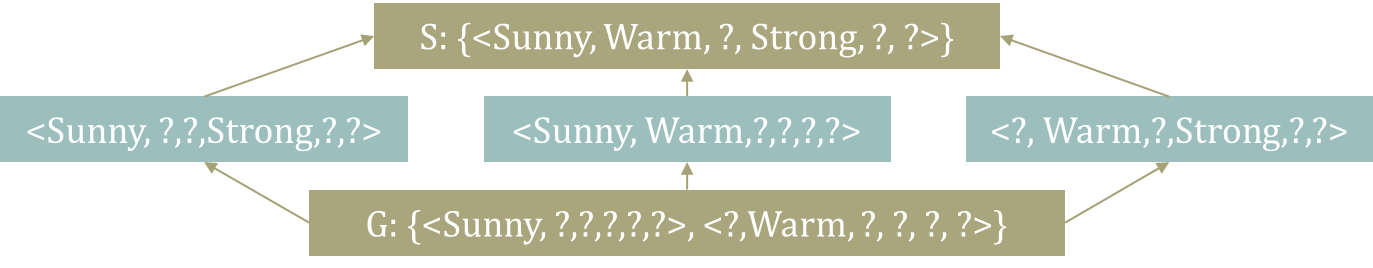
\includegraphics[scale=0.5]{Function_Approximation3.png}
\caption{물놀이 예제에서의 Version Space와 두 가지 Boundary}
\label{Figure 2-4}
\end{figure}

\begin{figure}[ht]
\centering
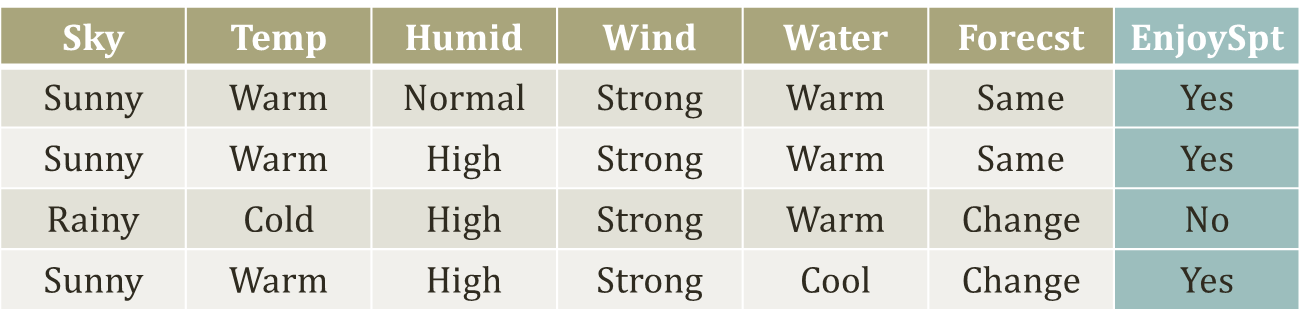
\includegraphics[scale=0.5]{Table1.png}
\caption{날씨나 기상예보에 따른 야외 물놀이 여부}
\label{Figure 2-5}
\end{figure}

%슬라이드10
\subsection{Candidate Elimination 알고리즘}
Candidate Elimination 알고리즘은 가장 일반적인 가설을 서서히 구체화시키고, 가장 구체적인 가설을 서서히 일반화시켜 두 가설 사이의 Version Space를 찾아내는 알고리즘이다. 좀 더 설명하자면, \\
\indent\rule{10cm}{0.4pt} \\
\begin{algorithm}[H]
	\SetAlgoLined
	\KwData{Training Dataset}
	\KwResult{Find the Version Space}
	Initialize $S$ = Maximally specific hypothesis $h$ in $H$
	Initialize $G$ = Maximally general hypothesis $h$ in $H$
	\For{instance $x$ in $D$}{
		\eIf{$y$ of $x$ is positive}{
			Generalize $S$ as much as needed to cover $o$ in $x$ \\
			Remove any $h$ in $G$, for which $h(o) \ne y$
		}{}
		\eIf{$y$ of $x$ is negative}{
			Specialize $G$ as much as needed to exclude $o$ in $x$ \\
			Remove any $h$ in $S$, for which $h(o) = y$
		}{}
	}
	Generate $h$ that satisfies $\exists s \in S, \exists g \in G, g \geq h \geq s$
\end{algorithm}

\indent\rule{10cm}{0.4pt} \\
\indent $S$와 $G$를 각각 가장 구체적인 가설, 가장 일반적인 가설로 초기화하고, 모든 인스턴스 $x \in D$에 대해 다음 과정을 반복한다; 만약 $x$의 Class Variable인 $y$가 positive이면, $S$가 해당 Attribute $o$를 충분히 포함할 수 있도록 일반화시키고, $G$에서 $h(o) \ne y$인 가설 $h$를 모두 빼준다. 만약 $x$의 Class Variable $y$가 negative이면, $S$와 $G$를 바꾸어 위와 같은 과정을 실행한다. 데이터의 모든 인스턴스에 대해 이 과정을 실행하고 나면, $S$와 $G$ 사이의 가설들을 찾는다.

%슬라이드11
\subsubsection{Candidate Elimination의 과정}
\begin{figure}[ht]
\centering
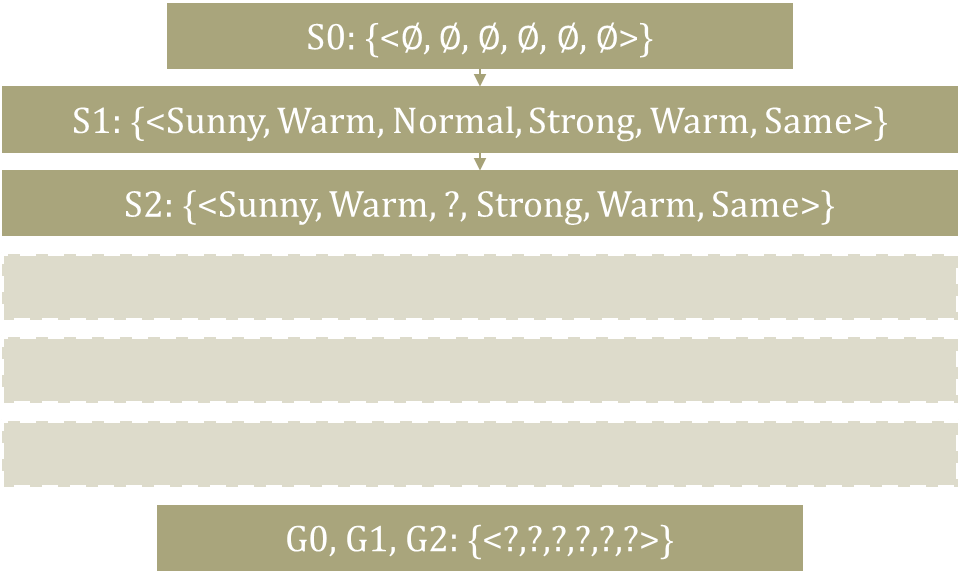
\includegraphics[scale=0.5]{Candidate_Elimination1.png}
\caption{Candidate Elimination Process 1}
\label{Figure 2-7}
\end{figure}
\indent 위의 그림에서 $S_{0}$는 가장 구체적인(절대로 물놀이를 나가지 않는) 가설, $G_{0}$는 가장 일반적인(무조건 나가서 물놀이를 즐기는) 가설에 해당한다. 표에서 첫 번째 인스턴스(첫 행)을 이용하여 $S_{0}$을 한 단계 일반화시킨다. 그 결과가 $S_{1}$에 해당하고, 두 번째 인스턴스(두 번째 행)를 이용하여 한 번 더 일반화시키면 $S_{2}$를 얻을 수 있다. 습도는 두 인스턴스가 각각 다른 값을 가지므로 ''?''로 두어 이 항목에 대해 영향을 받지 않도록 설정한다. 반면 나머지 항목들은 두 인스턴스에서 모두 일치하므로, 그 값을 그대로 가져온다. 이처럼 EnjoySport 결과값이 Positive인 경우는 $G_{0}$에는 영향을 주지 않으므로 $G_{1}$과 $G_{2}$는 업데이트되지 않는다. \\
\begin{figure}[ht]
\centering
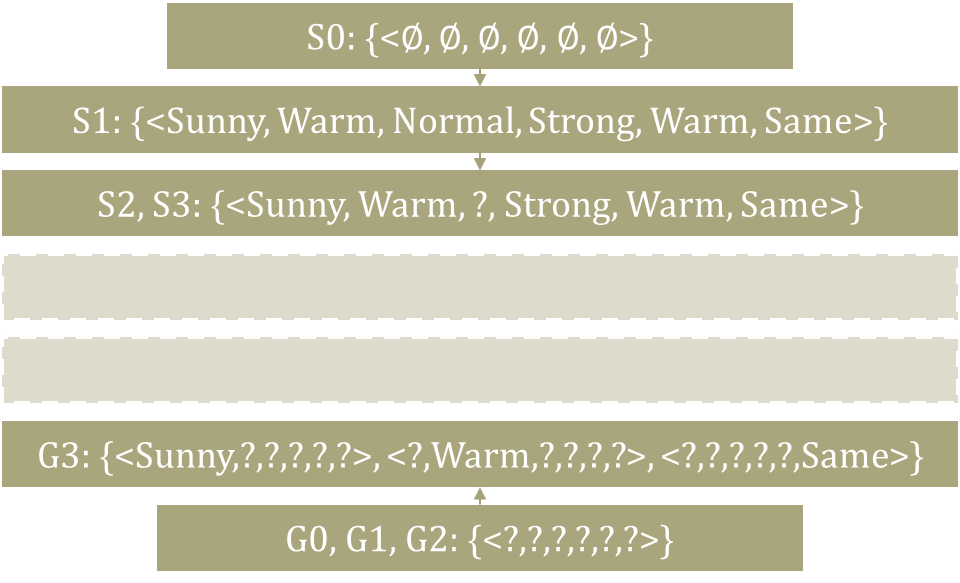
\includegraphics[scale=0.5]{Candidate_Elimination2.png}
\caption{Candidate Elimination Process 2}
\label{Figure 2-8}
\end{figure}
\indent 세 번째 인스턴스와 같이 나가서 놀지 않는 Negative Case는 $S_{2}$에는 영향을 주지 않으므로 $S_{3}$는 업데이트되지 않는다. 반면 $G_{0}$는 항상 나가서 노는 가설이므로, 적어도 이 negative 인스턴스의 feature에 대해서는 부정하여 $G_{0}$를 좀 더 구체화시켜야 한다. 따라서 이 인스턴스의 하늘의 상태인 Rainy를 부정하는 Sunny로 $G_{0}$를 구체화시키거나, 기온 Cold를 부정하는 Warm으로 구체화시키거나, 혹은 일기예보 Change를 부정하는 Same으로 구체화시켜야 한다. (그림에서 $G_{3}$ 세 개) \\
\begin{figure}[ht]
\centering
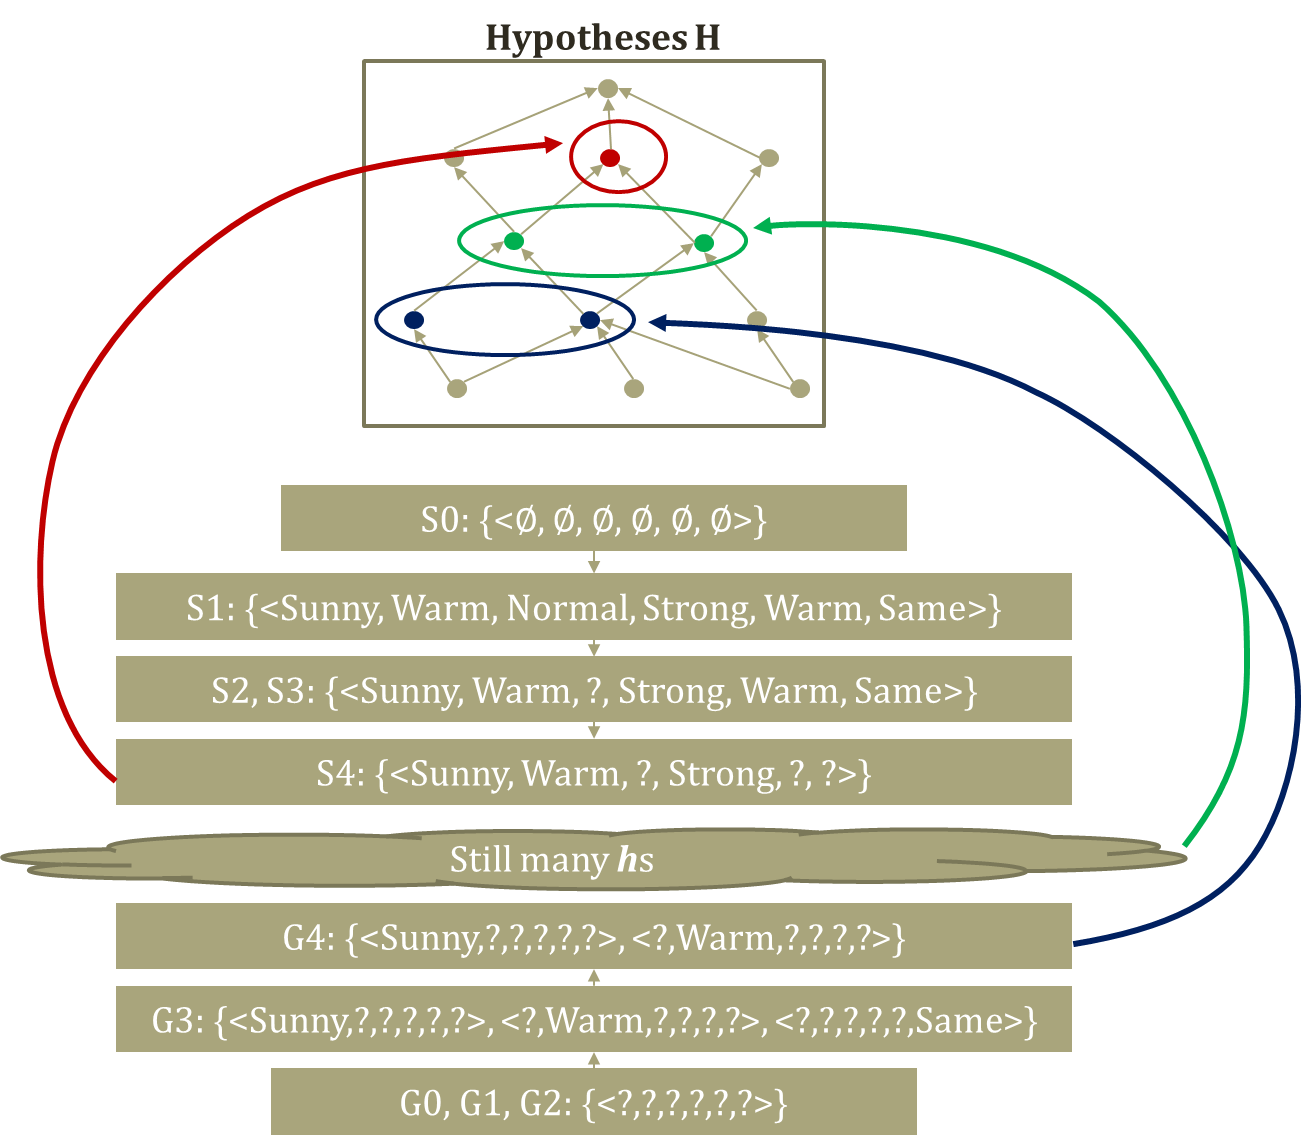
\includegraphics[scale=0.5]{Candidate_Elimination3.png}
\caption{Candidate Elimination Process 3}
\label{Figure 2-9}
\end{figure}
\indent 네 번째 인스턴스는 다시 Positive Case로 돌아왔다. Sunny, Warm, High, Strong 등 첫 4개 항목은 $S_{3}$에 영향을 주지 않음을 알 수 있다. 하지만 수온과 일기예보는 Cool, Change로서 기존의 인스턴스와 반대되는 값을 가지기 때문에, $S_{4}$는 마지막 두 항목에 대해 영향을 받지 않는 ''?''로 두어야 한다. 한편, 이 인스턴스는 일기예보  항목의 값이 'Change' 임에도 불구하고 Positive Case에 해당하므로 $G_{3}$에서 마지막 가설을 제거하여 $G_{4}$로 업데이트 한다. \\
\indent 여기까지 4개의 인스턴스를 이용하여 Specific Boundary를 일반화하고, General Boundary를 구체화하여 Version Space를 찾는 방법을 살펴보았다. 이 두 Boundary 사이에는 여전히 수많은 가설들이 존재할 수 있으며, 이들 중 우리가 찾고자 하는 목표함수가 있을 것이다. 이와 같은 학습을 통해 Version Space를 좁혀나가서 True Function을 찾아내는 방법을 Candidate Elimination Algorithm이라고 하는 것이다. \\

%슬라이드12
\subsubsection{How to Classify the Next Instance?}
\begin{figure}[ht]
\centering
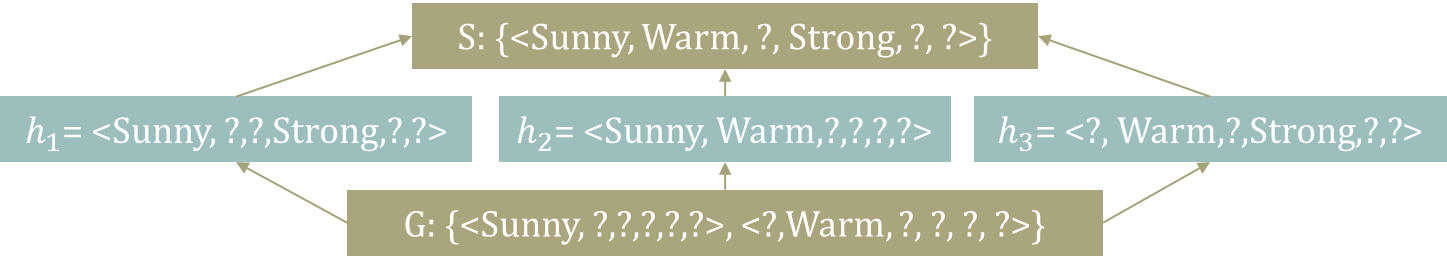
\includegraphics[scale=0.5]{Candidate_Elimination4.png}
\caption{asdf}
\label{Figure 2-10}
\end{figure}
일련의 규칙기반 학습을 통해 위 그림과 같은 Version Space를 얻었다고 가정해보자. 그리고, 다음의 인스턴스들을 가져와서 이 가족이 야외에서 물놀이를 즐길지 말지를 판별한다면 어떨까?
\begin{itemize}\setlength\itemsep{-\parsep}
	\item $<$Sunny, Warm, Normal, Strong, Cool, Change$>$
	\item $<$Rainy, Cold, Normal, Light, Warm, Same$>$
	\item $<$Sunny, Warm, Normal, Light, Warm, Same$>$
\end{itemize}

\indent 첫 번째 인스턴스는 가장 구체적 가설인 Specific Boundary의 가설을 만족시키므로 이 경우 야외 물놀이를 즐길 것이다. 두 번째 인스턴스는 가장 일반적 가설인 General Boundary의 가설들을 단 하나도 만족시키지 못하므로 야외 물놀이를 즐기지 않을 것이라 판별할 수 있다. 하지만 마지막 세 번째 인스턴스는  목표함수가 $h_{1}$이라면 ''No'', $h_{2}$라면 ''Yes'', $h_{3}$라면 ''No''의 값을 가지므로, 우리가 가지고 있는 Version Space로 결론내릴 수 없다. 따라서 더 많은 데이터를 가져와서 학습시켜야만 이 인스턴스를 판별할 수 있을 것이다. \\

\subsubsection{Candidate Elimination 알고리즘의 효용성}
Candidate Elimination 알고리즘이 실제로 잘 작동하는가? 라고 묻는다면, 이 장의 초반부에 제시한 이상세계의 세 가지 조건들을 만족시킨다면 '그렇다'고 대답할 수 있다. 하지만 실제 세계는 이 조건들을 모두 다 만족시키지는 못한다. 우리가 관측한 항목들 외에 결과에 영향을 미칠 수 있는 항목이 빠졌을 수도 있고, 중요한 항목들이 모두 반영되었다고 하더라도 관측 오차 등의 잡음(Noise)이 있을 수 있다. 따라서 실제로는, True function $h$가 오차를 포함한 데이터에 의해 걸러져버릴 수 있는 것이다.

%슬라이드 16
\section{의사결정 나무(Decision Tree)}

%슬라이드 17
\subsection{잡음(Noise)의 개입}
1장의 마지막 부분에서 언급했듯이 실제 세계에서는 거의 모든 데이터에 잡음(Noise)이 들어있는데, 규칙기반적 접근을 이용할 경우, 이러한 잡음은 목표함수를 찾아내는 데에 심각한 오류를 초래할 수 있다. 그렇다면 Noise를 포함하고 있는 데이터를 이용하면서 목표함수를 찾아낼 방법은 없을까? \\
\indent 통계적인 방법을 적절히 이용하여 Noise를 포함한 데이터를 통해 학습시킬 수 있는 방법이 바로 의사결정 나무(Decision Tree) 방법이다. 규칙기반 학습에서 보았던 물놀이 예제를 다시 상기하고, 다음 그림을 살펴보자. \\
\begin{figure}[ht]
\centering
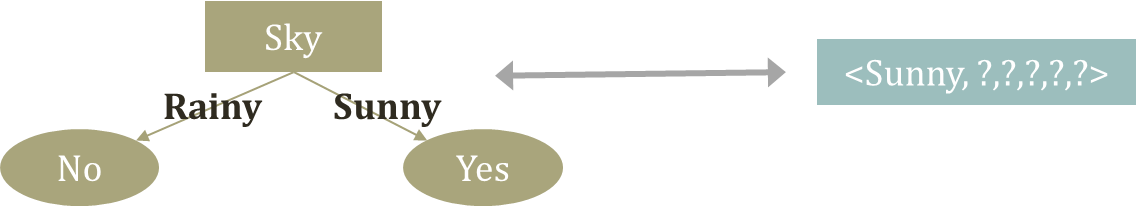
\includegraphics[scale=0.5]{Decision_Tree1.png}
\caption{의사결정 나무 예시}
\label{Figure 2-11}
\end{figure}
\indent 가설 $<$Sunny, ?, ?, ?, ?, ?$>$은 왼쪽과 같은 그림으로 표현할 수 있다. 이는 ''하늘이 맑으면 다른 조건들에 상관없이 무조건 나가서 물놀이를 한다.''는 가설이다. 여기서 사각형은 항목의 값이 정해질 수 있는 노드(Node)이고 타원은 최종 결과값을 나타내는 노드이다. 다음의 또 다른 예제를 보고 의사결정 나무와 이에 대응하는 가설을 확인하고 넘어가도록 하자.
\begin{figure}[ht]
\centering
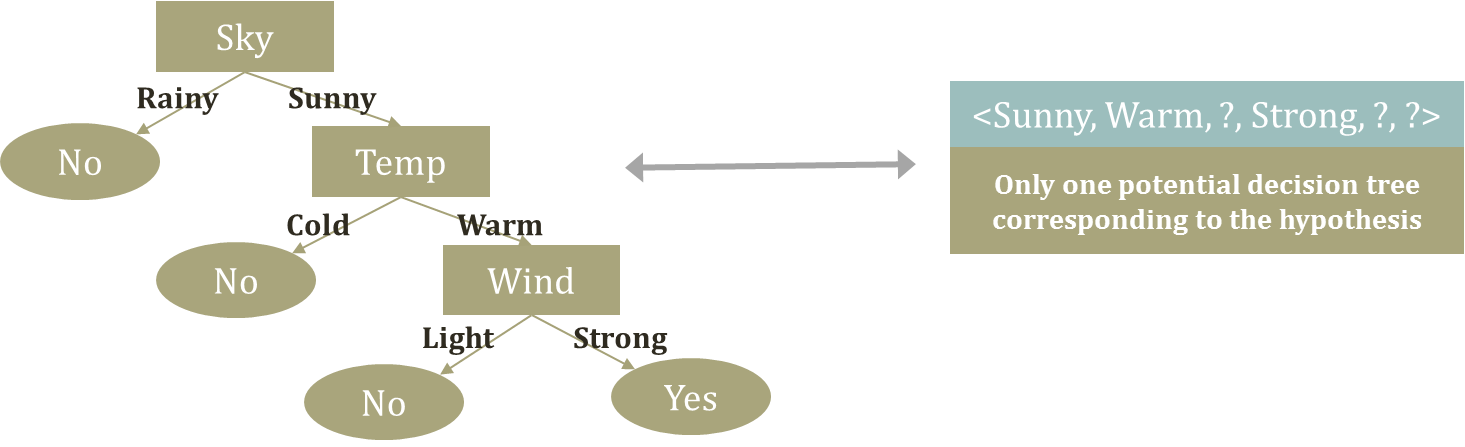
\includegraphics[scale=0.6]{Decision_Tree2.png}
\caption{의사결정 나무 예시2}
\label{Figure 2-12}
\end{figure}

%슬라이드 18
\subsection{신용평가 데이터를 이용한 예제}
기계학습 알고리즘의 성능을 확인할 때 많이 쓰이는 벤치마크 데이터 중에서, UCI신용평가 데이터(Credit Approval Dataset)를 이용한 다음의 예제를 살펴보자. 이 데이터는 총 690개의 인스턴스로 이루어져 있고, 이는 다시 307개의 Positive Case(허가)와 383개의 Negative Case(불허)로 나뉘어진다. 그리고 Attribute(특성)라고 불리는 각 고객의 특성을 나타내는 15개의 항목들과(A1 $\sim$ A15) Class Attribute(신용평가의 결과값)가 각각의 인스턴스를 구성하고 있다. 그 중 A1과 A9 두 항목을 기준으로 다음을 살펴보자. \\
\begin{figure}[ht]
\centering
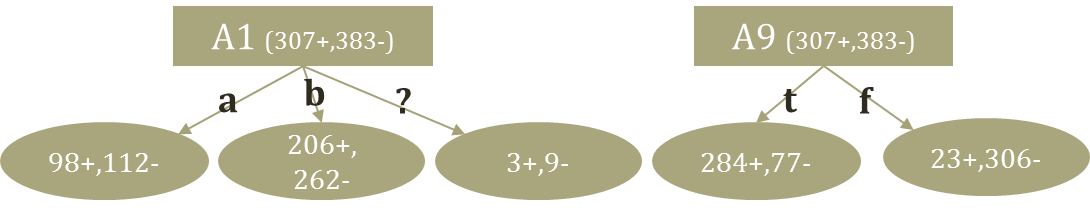
\includegraphics[scale=0.6]{Decision_Tree3.png}
\caption{UCI 신용평가 데이터에서 A1과 A9 Attribute의 분포}
\label{Figure 2-13}
\end{figure}
\indent 총 307개의 Positive Case 중 98개의 인스턴스는 A1 항목에 대해 $\textbf{a}$라는 값을, 206개는 $\textbf{b}$값, 3개는 무응답(''\textbf{?}'')이었고, 남은 383개의 Negative Case는 112개의 인스턴스가 A1 항목에 대해 $\textbf{a}$ 값, 262개는 $\textbf{b}$, 9개가 무응답(''\textbf{?}'')이었다. 마찬가지로 전체 690개의 인스턴스를 A9을 기준으로 나누어보자. 307개의 Positive Case는 284개는 A9에 대해 $\textbf{t}$값을 가졌고, 나머지 23개는 $\textbf{f}$값을 가졌다. 383개의 Nagative Case는 77개의 $\textbf{t}$값과 306개의 $\textbf{f}$값을 가졌다. 이를 나무(Tree) 구조로 표현하면 위와 같이 나타낼 수 있다. \\
\indent 만약 한 은행 직원이 15개의 특성 중 A1 하나만을 이용하여 class attribute 값을 추정한다면 어떨까? 예를 들어 A1 값이 $\textbf{a}$일 때, 무조건 positive case라고 분류한다면 이 직원은 98건은 올바르게 분류하지만 112건은 틀리게 된다. (반대로 A1이 $\textbf{a}$일 때 negative case로 분류하면 98건은 틀리고 112건만 맞출 것이다.) A1이 $\textbf{b}$일 때 positive 혹은 negative로 분류하더라도 상황은 비슷하다. 206건을 맞추는 대신 262건을 틀리거나, 혹은 262건은 맞추는 대신 206건은 틀리게 된다. A9 특성을 이용하여 분류한다면 어떨까? A9 값이 $\textbf{t}$일 때, positive case로 분류한다면 77건은 틀리지만, 그래도 284건은 올바르게 분류할 수 있다. 비슷하게 A9이 $\textbf{f}$일 때 negative case로 분류하면 23건은 틀리지만 306건은 맞추게 된다. 따라서, 오직 1개의 특성(Attribute)만 이용한다면, A1보다는 A9을 이용하는 게 훨씬 더 정확하다고 할 수 있다. \\

%슬라이드 19
\subsection{엔트로피}
그렇다면 앞의 예제와 같이 특정 Attribute를 이용하여 분류 작업을 함에 있어서 어떻게 하면 불확실성을 가장 많이 줄일 수 있을까? 혹은, 어떤 Attribute를 기준으로 이용해야 가장 정확하게 분류할 수 있을까? 이 질문에 대한 답을 하기 위해서는 Feature Variable의 불확실성(Uncertainty)을 수치화할 수 있어야 한다. \\
\indent 엔트로피란 열역학에서 사용하는 열역학적(혹은 통계역학적) 엔트로피의 개념을 가져온 것으로서, 열역학에서는 단일계 $i$의 상태에 대한 확률을 $p_{i}$라고 했을 때, 다음과 같이 정의한다; ($k_{B}$는 볼츠만 상수)
\begin{equation}
S = -k_{B}\sum p_{i}logp_{i} \tag{2-2}
\end{equation}

\indent 우리가 필요한 불확실성은 ''정보 엔트로피''로서, 클로드 섀넌(Claude Elwood Shannon)이 1948년 발표한 논문 $<$A Mathematical Theory of Communication$>$에서 제시한 개념이다. 어떤 확률변수(Random Variable) $X$가 어떤 확률분포(Probability Distribution) $P(X=x)$를 따를 때, 정보 엔트로피 $H(X)$는 다음과 같이 정의한다;
\begin{equation}
H(X) = -\sum_{X}P(X=x)log_{b}P(X=x) \tag{2-3}
\end{equation}

\indent 이와 같이 정의하였을 때, 엔트로피 값이 높다는 것은 불확실성이 높다는 것을 의미한다. 이를 시각적으로 보기 위해, 확률변수 $X$가 베르누이 분포(Bernoulli Distribution)를 따를 때 $P(X=1)$의 값이 변함에 따라 엔트로피 $H(X)$가 어떻게 변화하는지 그래프를 통해 살펴보자. 
\begin{figure}[ht]
\centering
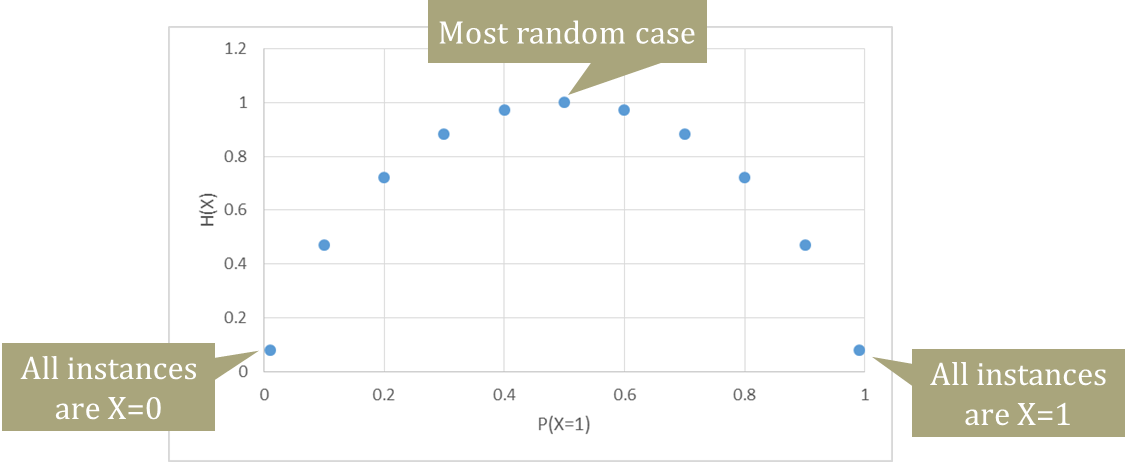
\includegraphics[scale=0.7]{Entropy.png}
\caption{베르누이 분포의 엔트로피}
\label{Figure 2-14}
\end{figure}

\indent 우리는 계속 이산적인(Discrete) 경우에 대해서만 다루겠지만, 만약 확률변수 $X$가 연속적인(Continuous) 확률변수라면, 엔트로피 정의의 합 기호를 적분기호로 바꾸고 Probability Function $P(X=x)$를 Probability Density Function $f(X=x)$로 바꿔주기만 하면 된다.

\subsubsection{조건부 엔트로피}
1단원에서 조건부 확률에 대해 배웠던 것을 상기해보자. 단순 엔트로피를 보기보다는 특정 Feature Variable의 값이 주어져있을 때의 엔트로피, 즉 조건부 엔트로피를 보는 것이 더 의미 있을 때가 많다. 조건부 엔트로피는 다음과 같이 정의한다;
\begin{align}
H(Y|X)	&= -\sum_{X}P(X=x)H(Y|X=x) \tag{2-4} \\
			&= \sum_{X}P(X=x)\{ -\sum_{Y}P(Y=y |X=x)log_{b}P(Y=y |X=x)\} \tag{2-5}
\end{align}

\indent $H(Y|X=x)$는 $X$의 값이 $x$로 정해져있을 때의 $Y$의 불확실성를 의미하는데, 이는 다시 $Y$에 대한 합으로 전개될 수 있다. 최종적으로 조건부 엔트로피는 ''$X=x$일 때 확률변수 $Y$의 엔트로피를 $P(X=x)$로 비중(weight)을 곱해 더한 값''이 된다.

%슬라이드 20
\subsubsection{정보 이득(Information Gain)}
\begin{figure}[ht]
\centering
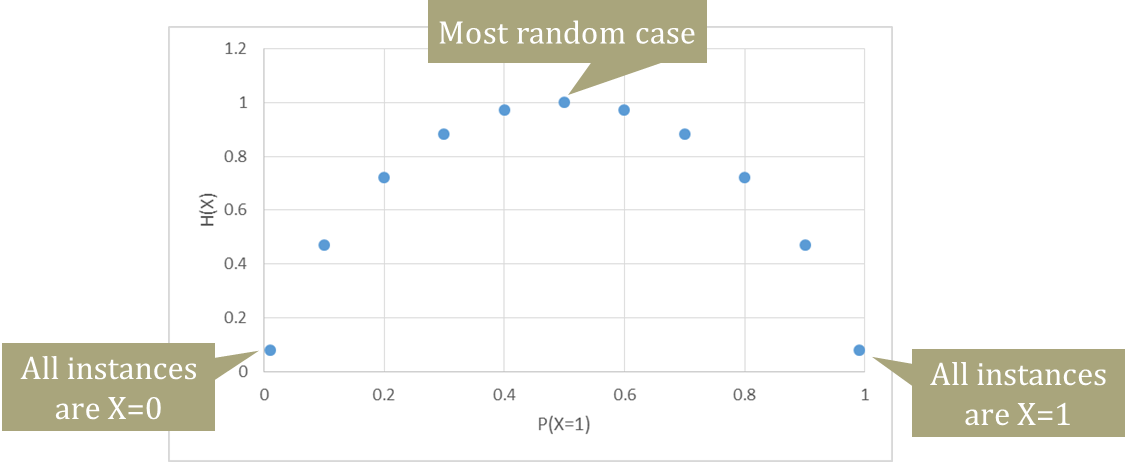
\includegraphics[scale=0.6]{Entropy.png}
\caption{각 노드에서의 엔트로피}
\label{Figure 2-15}
\end{figure}

\indent 앞서 정의한 엔트로피를 계산할 수 있는 Feature Variable에는 A1, A9 및 Class Variable이 있음을 알 수 있다. $Y$를 positive, negative case로 나누는 class variable이라고 하고, 각각 A1과 A9이 주어져있을 때의 조건부 엔트로피를 계산해보자.
\begin{flalign}
H(Y) &= -\sum_{Y \in \{ +,- \}}P(Y=y)log_{2}P(Y=y) \tag{2-6} \\
H(Y|A1) &= -\sum_{X \in \{ a, b, ? \}} \sum_{Y \in \{ +,- \}}P(A1=x, Y=y)log_{2}\frac{P(A1=x)}{P(A1=x, Y=y)} \tag{2-7} \\
H(Y|A9) &= -\sum_{X \in \{ t, f \}} \sum_{Y \in \{ +,- \}}P(A9=x, Y=y)log_{2}\frac{P(A9=x)}{P(A9=x, Y=y)} \tag{2-8}
\end{flalign}

\indent 식 (2-6)은 어떤 조건도 없이 $Y$ 변수에 대한 엔트로피를 계산하는 식이고, (2-7)과 (2-8)은 각각 A1과 A9에 대한 정보를 알고 있을 때의 조건부 엔트로피를 계산하는 식이다. (음의 부호로 로그의 분모 분자를 뒤집은 형태)
\indent 이 때, $A_{i}$ 변수로부터 얻은 정보이득(Information Gain) $IG(Y, A_{i})$는 $Y$ 변수의 엔트로피에서 $Y$의 $A_{i}$ 에 대한 조건부 엔트로피를 뺀 값으로 정의한다. 즉, 기존의 불확실성에서, 새로운 정보 $A_{i}$ 가 생겼을 때의 불확실성 만큼을 차감한 것이다. 위의 예제에서는 A9 변수의 값이 주어진다면, 더 높은 확률로 Class Variable을 추측할 수 있으므로, $Y$의 $A_{9}$에 대한 조건부 엔트로피가 $A_{1}$에 대한 조건부 엔트로피보다 더 낮음을 알 수 있다. 따라서 $A_{9}$ 변수의 정보이득(Information Gain)이 더 큰 값을 가진다.

%슬라이드 21
\subsection{Top-Down Induction Algorithm}
학습 과정에 있어서 의사결정 나무를 생성하는 방법에는 아주 다양한 방법이 있다. 대표적으로는 ID3, C4.5, CART 등이 있으나 여기서는 ID3 알고리즘만 간단하게 소개하고 넘어갈 것이다. \\
\textbf{ID3 알고리즘} \\
\indent\rule{10cm}{0.4pt} \\
\begin{algorithm}[H]
	\SetAlgoLined
	\KwData{Training Dataset}
	\KwResult{Create the corresponding Decision Tree}
	Initialize; Create an initial open node \\
	Initialize; Put instances in the initial node \\
	\While{There exists an open node}{
		Select an open node to split \\
		Select a best variable to split \\
		\For {Values of the selected variable}{
			Sort instances with the value of the selected variable \\
			Put the sorted items under the branch of the value of the variable \\
			\If {The sorted items are all in one class}{
				Close the leaf node of the branch
			}{}
		}
	}
\end{algorithm}

\indent\rule{10cm}{0.4pt} \\
\indent 우선 최초의 열린 노드(Initial Open Node) 생성하고, 이 노드에 모든 인스턴스 데이터를 입력한다. 그리고 모든 열린 노드를 다 닫을 때까지 다음 과정을 반복하는 것이다. \\
\indent (1) 열린 노드를 선택하고,\\
\indent (2) 이 노드를 하위 노드들로 쪼개기에 가장 적합한 변수를 탐색(Ex. 정보이득이 가장 큰 변수)한 뒤,\\
\indent (3) 선택된 변수에 대해 다음을 실행: \\
\indent \indent (3-1) 위에서 고른 변수값에 따라 모든 인스턴스를 정렬,\\
\indent \indent (3-2) 정렬된 인스턴스들을 변수값을 기준으로 나누어 한 단계 아래의 노드(Child Node)들을 생성\\
\indent \indent (3-3) 만약 모든 인스턴스가 하나의 가지에 다 들어가면;\\
\indent \indent \indent (3-3-1) 해당 잎 노드(Leaf Node)를 닫고 다음으로 진행\\

%슬라이드 22
\textbf{의사결정 나무 예시}
\begin{figure}[ht]
\centering
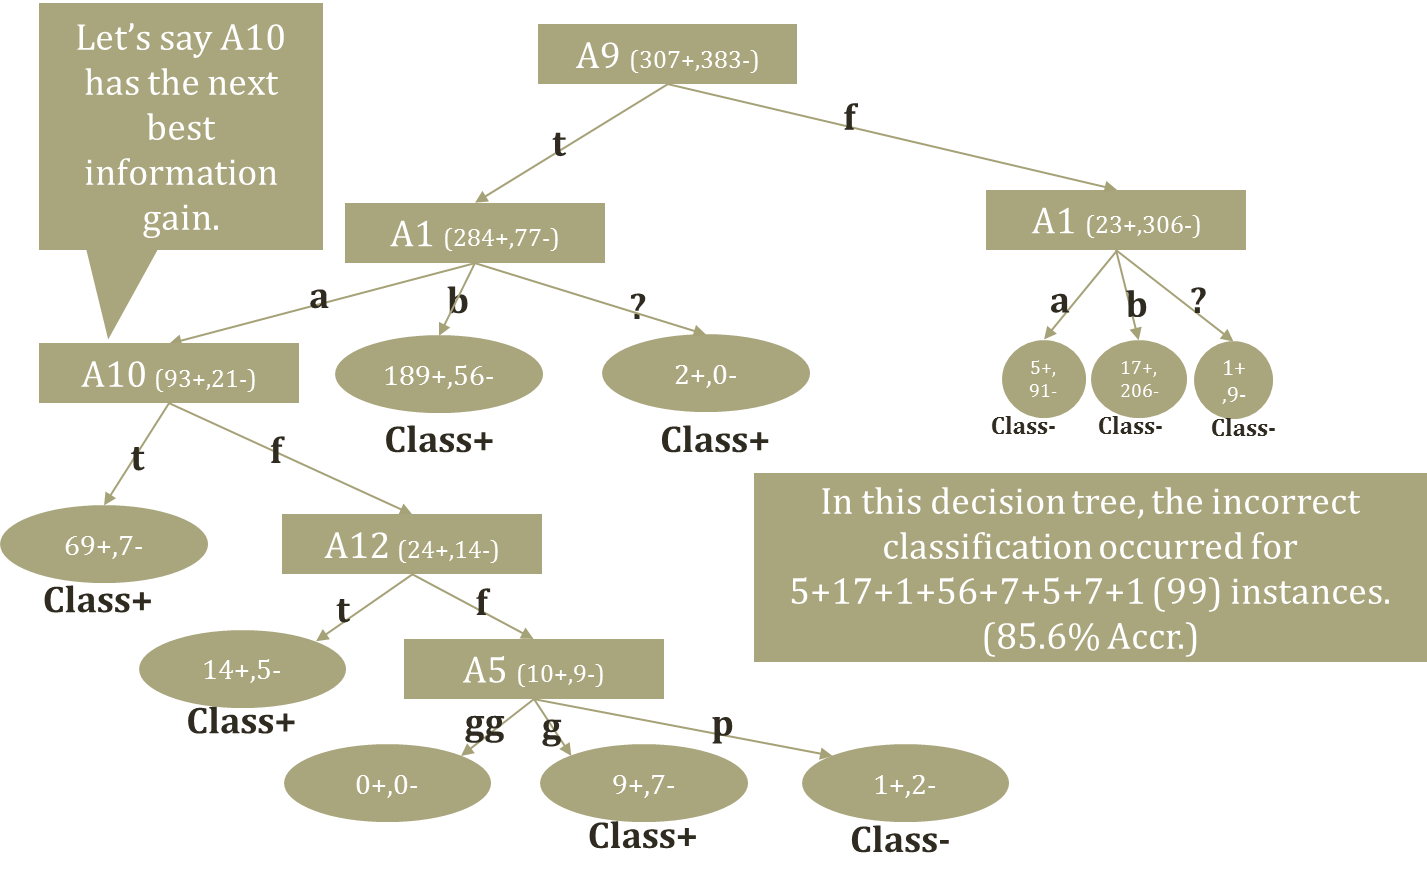
\includegraphics[scale=0.6]{Decision_Tree4.png}
\caption{신용평가 예제의 의사결정 나무}
\label{Figure 2-16}
\end{figure}

\indent 위 그림은 A1, A9 Attribute 이외에도 A10, A12, A5 등을 더 사용하여 의사결정 나무를 확장시킨 것이다. A9 항목의 값이 $\textbf{t}$이면 A1 항목에 따라 데이터를 분류하는데, A1이 $\textbf{b}$이거나 \textbf{?}이면 Class Variable을 \textbf{+}로 분류하고, A1이 $\textbf{a}$이면 다시 A10 항목을 이용하여 더 세부적으로 나눈다. 이 때 A10 항목이 남은 Feature Variable 중에서 정보이득이 가장 큰 항목이라고 생각할 수 있다. \\
\indent 이 결정 나무는 대체적으로 잘 작동하는 것처럼 보이지만, A9이 $\textbf{t}$이고, A1이 $\textbf{b}$이면 189건에 대해서는 맞지만 56건에 대해서는 틀린 분류를 하게 된다. 따라서 56건에 대해서도 더 정확한 분류를 하고 싶다면 더 많은 Feature Variable을 이용해서 나무를 확장시켜 나가야 한다. 이렇게 하면, 적어도 우리가 가지고 있는 데이터에 대해서는 아주 잘 작동하는 의사결정 나무를 생성할 수 있다.

%슬라이드 23
\subsection{의사결정 나무 방법의 한계}
앞서 언급했듯이, 의사결정 나무는 주어진 데이터에 대해서 아주 정확하게 작동하도록 잘 생성될 수 있다. 그 방법은 단순하게, 데이터에 포함된 모든 Attribute를 이용하는 것이다. 하지만 이렇게 나무의 크기를 증가시킨다고 해서 반드시 좋은 것은 아니다. 크기가 큰 나무를 현실세계에 적용해보면 오히려 적당한 크기의 나무보다 잘 작동하지 않을 때가 많다. 이는 여러가지 잡음(Noise)과 서로 모순적인 Inconsistent한 데이터 때문인데, 실제로는 이러한 요소들이 많이 포함될 수밖에 없다. 아래의 그래프를 보면, 결정나무의 크기가 계속해서 증가할 때, 우리가 가지고 있는 훈련 데이터(Training Dataset)에 대해서는 정확도가 계속 올라가지만, 테스트 데이터(Test Dataset)에 대해서는 정확도가 어느정도 올라가다가 일정 선을 넘으면 오히려 떨어지는 것을 관찰할 수 있다.
\begin{figure}[ht]
\centering
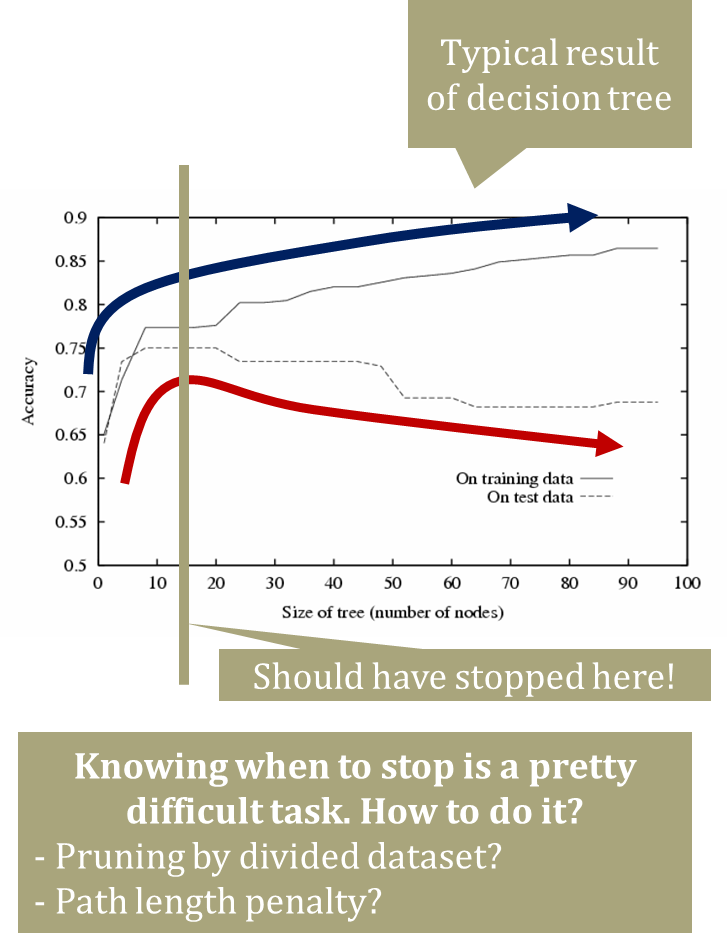
\includegraphics[scale=0.6]{Decision_Tree_Weakness.png}
\caption{의사결정 나무의 크기와 성능}
\label{Figure 2-17}
\end{figure}

%슬라이드 24
\subsection{규칙기반 학습의 한계}
이 단원의 앞부분에서 다루었던 Find-S 알고리즘과 Candidate-Elimination 알고리즘, 그리고 의사결정 나무 방법은 모두 규칙기반(Rule-based) 학습에 해당한다. 규칙기반 기계학습은 실행하기가 쉽고, 이를 이용하는 사람도 쉽게 이해할 수 있다는 장점이 있다. 하지만 데이터가 이상적인 가정들을 만족해야 하고, 단 하나라도 기존의 관측과 모순적인 데이터가 있으면 심각한 문제가 된다. 특히 Candidate-Elimination 알고리즘 등을 이용할 경우, True function으로 정확하게 수렴하려면 주어진 데이터가 모든 Feature Variable을 설명할 수 있도록 커야하고, 잡음에 의해서 이 목표함수가 제외될 위험성이 있다. 의사결정 나무를 이용할 경우, 어느정도 깊이(Depth)의 나무가 적절할지 판단하는 것도 쉽지 않다. \\
\indent 하지만 규칙기반 방법은 아직도 광범위하게 이용되고 있는데, 사용하기 쉽다는 접근성 때문이다. 하지만 데이터의 잡음과 상호 모순적인 데이터를 잘 다루어야만 이를 잘 적용할 수 있다.

%슬라이드 25
\section{선형회귀(Linear Regression)}

%슬라이드 26
\subsection{통계적 접근; 선형회귀}
이 장에서는 앞서 배운 규칙기반이나 의사결정 나무와 달리, 좀 더 통계학적인 접근을 취할 것이다. 이 부분에서 사용할 데이터는 UCI의 부동산 데이터인데, 이는 13개의 Attribute(Independent Variable)와 1개의 Dependent Value가 있는 형태이다. 여기서 독립변수와 종속변수는 모두 연속적인(Continuous) 값을 갖는데, 이는 앞서 UCI 신용평가 데이터에서 Class Variable처럼 \textbf{+}와 \textbf{-} 두 가지 값만 갖는 이산적인(Discrete) 값을 갖는 경우와 대조된다. \\
\indent 기계학습이란 본질적으로, Probably Approximately Correct한 목표함수를 학습하는 것이라고 할 수 있는데, 선형회귀는 그 함수를 선형함수(Linear Function)로서 근사하는 방법인 것이다. 따라서 가설 $h$는 다음과 같은 함수로 표현할 수 있다;
\begin{equation}
h: \hat{f}(x, \theta) = \theta_{0} + \sum_{i=1}^{n}\theta_{i} x_{i} = \sum_{i=0}^{n}\theta_{i} x_{i} \tag{2-9}
\end{equation}

\indent 즉, 목표함수를 Feature Variable의 선형적 가중치의 합(Linearly Weighted Sum)이라고 생각하는 것이다. 우리는 선형회귀 방법을 이용할 것이므로 선형 가정은 그대로 둔다면, 목표함수의 정확한 학습을 위해서는 매개변수(Parameter)인 $\theta_{i}$를 잘 학습하는 것이 핵심이라고 할 수 있다. $n$은 Feature Variable의 갯수를 의미한다.

%슬라이드 27
\subsubsection{선형회귀의 매개변수 \texorpdfstring{\textbf{$\theta$}}{Lg} 찾기}
앞서 보았던 가설 함수의 형태는 다시 행렬의 곱 형태로 나타낼 수 있는데, 데이터를 $m\times n$행렬도 표현하고, 매개변수 $\theta$를 $n \times 1$행렬(벡터)로 표현하면 다음과 같은 형태가 된다($n$개의 Feature Variable에 대해서, 총 $m$번의 관측치를 가지고 있는 것이다.);
\begin{equation}
h: \hat{f}(x, \theta) = \sum_{i=0}^{n}\theta_{i} x_{i} \to \hat{f}(x, \theta) = X\theta 			\tag{2-10}
\end{equation}
\begin{flalign}
X &= \begin{bmatrix}
1		&x_{1}^{1}	&\hdots	&x_{n}^{1} \\
1		&x_{1}^{2}	&\hdots	&x_{n}^{2} \\
\vdots 	&\vdots 	&\ddots 	&\vdots \\
1		&x_{1}^{m}	&\hdots 	&x_{n}^{m} \\
\end{bmatrix}
, \theta = \begin{bmatrix}
\theta_{0} \\ \theta_{1} \\ \vdots \\ \theta_{n} \\
\end{bmatrix}																			\tag{2-11}
\end{flalign}

\indent 여기서 $x_{i}$는 $i$번째 Feature Variable을 의미하고, 이 문자의 위첨자는 우리가 가지고 있는 데이터 중에서 몇번째 데이터인지를 나타내는 숫자이다. 하지만 현실세계에서는 데이터에 잡음(Noise)이 들어가게 되는데 이를 표현해주기 위해 True function $f(x, \theta)$에 $n \times 1$ 벡터인 $e$를 더해주게 된다;
\begin{equation}
h: f(x, \theta) = \sum_{i=0}^{n}\theta_{i} x_{i} + e \to f = X\theta + e = Y					\tag{2-12}
\end{equation}

\indent True function $f(x, \theta)$와 가설 $\hat{f}(x, \theta)$의 차를 오차(Error)라고 부르는데, 우리는 이 오차의 제곱(Squared Error)을 최소화하는 방법으로 매개변수 $\theta$를 찾을 것이다. 여기서 오차는 벡터 형태이므로 단순히 각 Component의 제곱의 합(또는 Euclidean Norm의 제곱)을 최소화하면 된다.
\begin{align}
\hat{\theta}	&= argmin_{\theta}(f - \hat{f})^{2} 											\tag{2-13}\\
			&= argmin_{\theta}(Y-X\theta)^{2} 											\tag{2-14}\\
			&= argmin_{\theta}(Y-X\theta)^{T}(Y-X\theta) 								\tag{2-15}\\
			&= argmin_{\theta}(\theta^{T}X^{T}X\theta - 2\theta^{T}X^{T}Y + Y^{T}Y) 	\tag{2-16}\\
			&= argmin_{\theta}(\theta^{T}X^{T}X\theta - 2\theta^{T}X^{T}Y) 			\tag{2-17}\\
\end{align}

\indent Argument Minimum과 Argument Maximum은 MLE와 MAP 부분에서 공부했던 것을 상기하자. 해당 식은 $(f - \hat{f})^{2}$의 값을 최소화시키는 $\theta$값을 의미한다. $Y = f(x;\theta)$, $\hat{f} = X\theta$이므로 식 (2-14)와 같이 표현되고, 이는 다시 (2-15), (2-16)처럼 나타낼 수 있다. 여기서 True function을 나타내는 $Y$를 포함한 항($Y^{T}Y$)은 여기서 $\theta$ 와는 무관하므로 $argmin_{\theta}$에서 사라질 수 있다.

%슬라이드 28
\subsubsection{\texorpdfstring{$\theta$}{Lg}의 최적값(Optimized Value)}
앞에서 보았듯이, $\hat{\theta} = argmin_{\theta}(\theta^{T}X^{T}X\theta - 2\theta^{T}X^{T}Y)$임을 확인하였다. 괄호 안의 식을 최소화하는 $\theta$의 값은 단순히 미분값이 0이 되는 지점에서 찾을 수 있다. 따라서,
\begin{equation} 
\nabla_{\theta}(\theta^{T}X^{T}X\theta - 2 \theta^{T}X^{T}Y) = 0						\tag{2-18}\\
\end{equation}
\begin{equation} 
\to 2 X^{T}X\theta - 2 X^{T}Y = 0														\tag{2-19}\\
\end{equation}
\begin{equation}
\to \theta = (X^{T}X)^{-1}X^{T}Y														\tag{2-20}\\
\end{equation}

\indent 간단한 벡터 미분을 통하여 (2-20)의 최종 결과를 얻을 수 있다! UCI 부동산 데이터에서 하나의 Feature Variable만 이용하여 선형회귀 함수의 결과를 살펴보자. x축은 사용한 Feature Variable의 값이고, y축은 Dependent Variable의 값이다. 빨간색 점은 실제 데이터의 분포이고, 파란색 선은 선형회귀 방정식의 그래프이다.
\begin{figure}[ht]
\centering
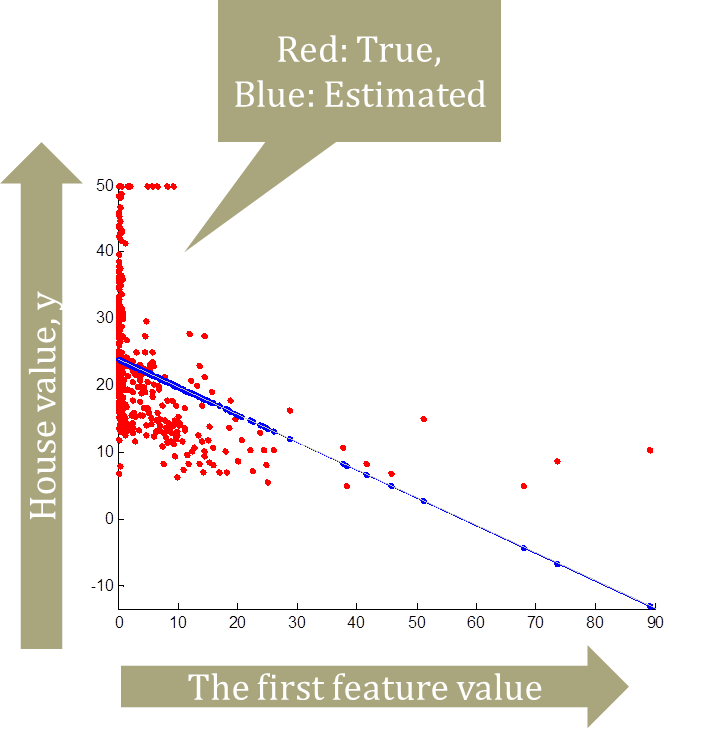
\includegraphics[scale=0.6]{Linear_Regression.png}
\caption{UCI 부동산 데이터의 선형회귀 결과}
\label{Figure 2-18}
\end{figure}

%슬라이드 29
\subsubsection{More Precise Regression}
앞서 본 선형회귀의 그래프는 왠지 잘 맞지 않는 것처럼 보인다. 특히 Feature Variable의 값이 아주 작을 때와 클 때는 애초에 선형의 그래프를 따르는 것 같지 않다. 이를 해결하기 위해 단순 선형회귀가 아닌 다항회귀(Polynomial Regression)를 이용하기도 하는데, $x$의 1차항만 고려하는 것이 아니라 $x^{2}, x^{3}, \hdots$ 등 고차항을 이용하는 것이다. 함수의 형태가 더 복잡해지므로 데이터를 설명하는 능력도 올라갈 것이다. 이를 식으로 나타내면 다음과 같다;
\begin{equation} 
h: \hat{f}(x;\theta)=\sum_{i=0}^{n}\sum_{j=1}^{m}\theta_{i,j}\phi_{j}(x_{i}) 				\tag{2-21}\\
\end{equation}
\begin{figure}[ht]
\centering
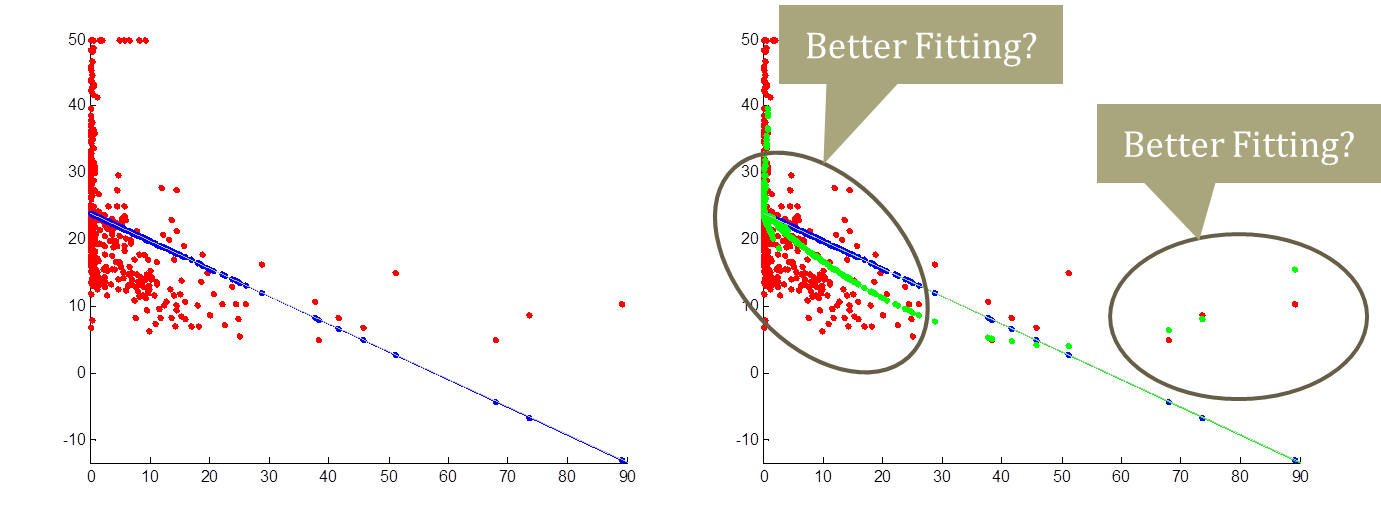
\includegraphics[scale=0.6]{Linear_Regression2.png}
\caption{UCI 부동산 데이터의 다항회귀 결과}
\label{Figure 2-19}
\end{figure}

\indent 왼쪽의 선형회귀 결과와 오른쪽의 다항회귀 결과(9차항까지 사용)를 비교해보자. 이 곡선 형태가 본래 데이터인 빨간 점들과 더 잘 맞는 것처럼 보인다. 하지만 x축의 오른쪽 부분에서 아주 소수의 관측값만 가지고 이 부분을 더 잘 설명하기 위해 차수를 늘리는 것이 타당한지는 고려해봐야 할 문제이다. 이것은 의사결정 나무에서 세세한 부분까지 더 정확하게 분류하기 위해 나무의 깊이(Depth)를 계속 더 늘리는 것과 근본적으로 같은 문제이다.

%슬라이드 30
\section*{정리하며}
여기까지 규칙기반(Rule-based), 의사결정 나무(Decision Tree), 선형회귀(Linear Regression) 등의 방법을 살펴보았다. 이 방법들은 매우 간단하며 아직도 여러 분야에서 많이 사용되고 있다. 하지만 데이터의 수가 많아지고 잡음이 많아질수록 오류가 많은 모델이기에 조심스럽게 접근해야 한다. 다음 단원에서는 마찬가지로 단순하면서 좀 더 통계적으로 접근하는 Naive Bayes Classifier에 대해 배워볼 것이다.

%슬라이드 31
\section*{Acknowledgement}
This material is greatly influenced by
\begin{itemize}\setlength\itemsep{-\parsep}
\item Professor Tom Mitchell at CMU \\
\item Professor Eric P. Xing at CMU
\end{itemize}

%슬라이드 32
\section*{Further Readings}
\begin{itemize}\setlength\itemsep{-\parsep}
\item Bishop Chapter 14.4 \\
\item Mitchell Chapter 1, 2, 3
\end{itemize}
\end{document}

%ALIGNING EQUATIONS
\begin{align}
0 	&= 3x^3+3x^2-6x 		\\
	&=3(x^3+x^2-2x) 		\label{three} \\
	&=3x(x^2+x-2) 		\label{x} \\
	&= 3x(x+2)(x-1) 		\label{linear} \\
	\therefore x &=0, -2, 1 \nonumber
\end{align} \\
In step (\ref{three}) I factored out a three.
In step (\ref{x}) I factored out an $x$.
In step (\ref{linear}) I factored out linear polynomials.

%FRACTION REPRESENTATION
A Fraction 		$\dfrac{x^4}{x^3(x-1)^2} = \dfrac{x}{(x-1)^2}$,	\\ \\
A Square Root 	$\sqrt{16} = \pm 4$,								\\ \\
An Integral 		$F(x) = \int_{a}^{b}f(x)dx$, 							\\ \\
The Quadratic Formula for $ax^2+bx+c=0$ is $x=\dfrac{-b\pm\sqrt{b^2-4ac}}{2a}$ \\ \\

%ARRANGEMENT
An Equation $x^2+\sqrt{y}=z-3$ which is inside the sentence is said to be arranged in-line. \\
An Equation like the following; $$F(x) = \int_{a}^{b}f(x)dx$$
is, however, arranged at the center of the paper.\\
\begin{align}
x^2+y^2 & =z^2	\\
&=\sin(x) + y		\\
&=x+y+q			\\
&=\sqrt{\frac{a}{b}}
\end{align}

%TABULAR
Let's take the function $f(x) = \sqrt{x^2+1}$ and make a table of vaules. \\
\begin{center}
\begin{tabular}{r|cccc}
$x$		& -1	& 0 & 1 & 2 \\
\hline
$f(x)$		& $\sqrt{2}$ & 1 & $\sqrt{2}$ & $\sqrt{5}$ \\
\end{tabular}
\end{center}

%Table2
\begin{table}[]
\centering
\begin{tabular}{ccccccc}
\rowcolor[HTML]{656565} 
{\color[HTML]{FFFFFF} \textbf{Sky}} & {\color[HTML]{FFFFFF} \textbf{Temperature}} & {\color[HTML]{FFFFFF} \textbf{Humidity}} & {\color[HTML]{FFFFFF} \textbf{Wind}} & {\color[HTML]{FFFFFF} \textbf{Water}} & {\color[HTML]{FFFFFF} \textbf{Forecast}} & \cellcolor[HTML]{C0C0C0}{\color[HTML]{333333} \textbf{Enjoy Sport}} \\
Sunny                               & Warm                                        & Normal                                   & Strong                               & Warm                                  & Same                                     & \cellcolor[HTML]{EFEFEF}{\color[HTML]{333333} Yes}                  \\
Sunny                               & Warm                                        & High                                     & Strong                               & Warm                                  & Same                                     & \cellcolor[HTML]{EFEFEF}{\color[HTML]{333333} Yes}                  \\
Rainy                               & Cold                                        & High                                     & Strong                               & Warm                                  & Change                                   & \cellcolor[HTML]{EFEFEF}{\color[HTML]{333333} No}                   \\
Sunny                               & Warm                                        & High                                     & Strong                               & Cool                                  & Change                                   & \cellcolor[HTML]{EFEFEF}{\color[HTML]{333333} Yes}                 
\end{tabular}
\caption{Figure 2-1}
\label{my-label}
\end{table}